\documentclass{standalone}
\usepackage[utf8]{inputenc}
\usepackage[T1]{fontenc}
\usepackage{tikz}
\usetikzlibrary{arrows.meta, positioning}

\begin{document}

\begin{center}
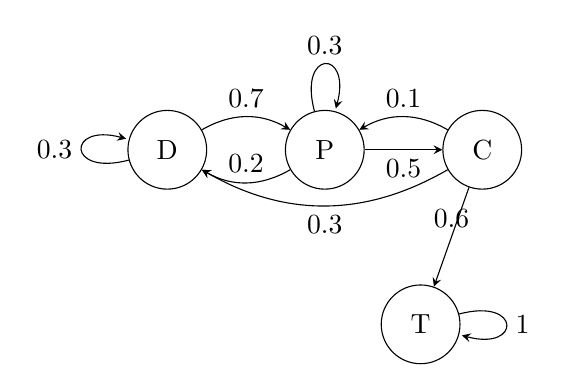
\begin{tikzpicture}[->, >=stealth, node distance=2cm, scale=1, transform shape,
    state/.style={circle, draw, minimum size=1cm, inner sep=0pt}]
  
  % Definir nodos
  \node[state] (D) {D};
  \node[state] (P) [right of=D] {P};
  \node[state] (C) [right of=P] {C};
  \node[state] (T) [below right=1.5cm and 0.5cm of P] {T};
  
  % Transiciones desde D
  \draw[bend left] (D) to node[above] {0.7} (P);
  \draw[loop left] (D) edge node[left] {0.3} (D);
  
  % Transiciones desde P
  \draw[bend left] (P) to node[above] {0.2} (D);
  \draw (P) to node[below] {0.5} (C);
  \draw[loop above] (P) edge node[above] {0.3} (P);
  
  % Transiciones desde C
  \draw (C) to node[above] {0.6} (T);
  \draw[bend left] (C) to node[below] {0.3} (D);
  \draw[bend right] (C) to node[above] {0.1} (P);
  
  % Transición desde T (autoloop)
  \draw[loop right] (T) edge node[right] {1} (T);
  
\end{tikzpicture}
\end{center}

\end{document}
